\documentclass[a4paper,11pt,eval]{nsi} 
\usepackage{pifont}
\usepackage{fontawesome5}

%\pagestyle{empty}


\newcounter{exoNum}
\setcounter{exoNum}{0}
%
\newcommand{\exo}[1]
{
	\addtocounter{exoNum}{1}
	{\titlefont\color{UGLiBlue}\Large Exercice\ \theexoNum\ \normalsize{#1}}\smallskip	
}



\begin{document}



\textcolor{UGLiBlue}{Vendredi 28/03/2025}\\
\classe{\premiere spé}
\titre{Evaluation-bilan 5}
\maketitle
\begin{center}
	Calculatrice autorisée. Toutes les réponses doivent être justifiées.
\end{center}

\vspace{1cm}


\exo{ Concentration d'un antibiotique}\bareme{8 pts}\\
On étudie la concentration dans le sang en fonction du temps d'un antibiotique injecté en une seule prise à un patient. On modélise cette concentration par la fonction $g$ définie sur l'intervalle $\fif{0}{10}$ par : $\quad g(t)=\dfrac{6t}{t^2+4}$.\\
$g(t)$ représente la concentration en mg.L$^{-1}$ de l'antibiotique lorsque $t$ heures se sont écoulées.\\[.5em]
Répondre aux questions suivantes de façon algébrique. Il est possible de vérifier la cohérence des résultats à l'aide d'un graphique à la calculatrice.
\begin{enumerate}
    \item On cherche à déterminer sur quel intervalle de temps la concentration sera supérieure ou égale à 1,2 mg.L$^{-1}$.
        \begin{enumalph}
            \item Montrer que résoudre l'inéquation $\quad g(t)\geqslant 1,2 \quad$ revient à résoudre l'inéquation\\ $\quad -1,2t^2+6t-4,8\geqslant 0$.
            \item Résoudre l'inéquation $\quad -1,2t^2+6t-4,8\geqslant 0\quad$ et conclure : sur quel intervalle de temps la concentration sera-t-elle supérieure ou égale à 1,2 mg.L$^{-1}$ ?
        \end{enumalph}
        \carreauxseyes{16cm}{8.8cm}\\
        \carreauxseyes{16cm}{12cm}

    \item On cherche à déterminer si concentration peut être strictement supérieure à 1,5 mg.L$^{-1}$.
    \begin{enumalph}
        \item Montrer que résoudre l'inéquation $\quad g(t)>1,5 \quad$ revient à résoudre l'inéquation\\ $\quad -1,5t^2+6t-6> 0$.
        \item Résoudre l'inéquation $\quad -1,5t^2+6t-6> 0\quad$ et conclure : la concentration peut-elle être strictement supérieure à 1,5 mg.L$^{-1}$ ?
    \end{enumalph}
    \carreauxseyes{16cm}{9.6cm}\\
    \carreauxseyes{16cm}{8cm}
\end{enumerate}

\vspace*{.5cm}

\dleft{8cm}{
    \exo{}\bareme{8 pts}\\
    La courbe ci-contre représente dans un repère du plan une fonction $f$ définie et dérivable sur l'ensemble des nombres réels.\\

    Les points A$(0~;-2)$ et B $(3~;11,5)$ appartiennent à  la courbe représentative de la fonction $f$ et les tangentes à  la courbe aux points A et B sont horizontales.\\

    Le but de l'exercice est de déterminer l'expression algébrique de la fonction $f$.
}{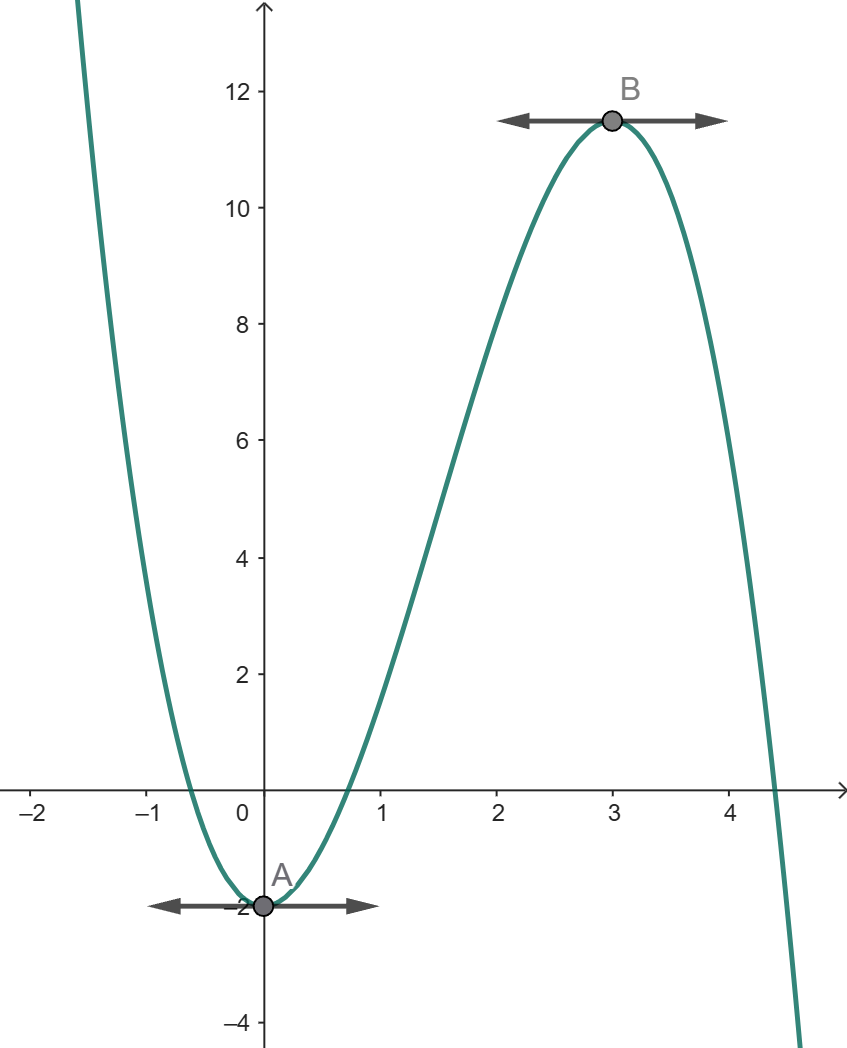
\includegraphics[width=8.4cm]{courbe4.png}}


\begin{enumerate}
\item Déterminer $f(0),\, f(3), f'(0)$ et $f'(3)$.\\[.5em]
\carreauxseyes{16cm}{4cm}\\
\item  On admet que pour tout réel $x$\,, $f(x)$ peut s'écrire sous la forme :
$$f(x) = ax^3 +bx^2 +cx +d,$$

où \: $a,\, b,\, c$ \: et\: $d$\: désignent des nombres réels .


	\begin{enumalph}
		\item Donner une expression de $f'(x)$ à l'aide de $a,b,c$ et $d$.\\[.5em]
        \carreauxseyes{16cm}{1.6cm}\\
    \item Traduire $f(0)=-2$ par une égalité sur les coefficients $a,b,c$ et $d$ et en déduire la valeur de $d$.
    Traduire $f'(0)=0$ par une égalité et en déduire la valeur de $c$.\\[.5em]
    \carreauxseyes{16cm}{4cm}\\
    Conclure : \\
    Pour tout $x\in \R, f(x)= ax^3+bx^2+ .........................\quad$ et $\quad f'(x)=$\dotfill
    \item Traduire $f(3)=11,5$ par une égalité sur les coefficients $a$ et $b$.\\
    Traduire $f'(3)=0$ par une égalité sur les coefficients $a$ et $b$.\\[.5em]
    \carreauxseyes{16cm}{4cm}\\
    \item Résoudre le système $\quad (S):\left\{
        \begin{array}{l}
            \ 27a+9b=13,5 \\
            \ 27a+6b=0 \\
        \end{array} \right.$\\[.5em]
    Conclure en donnant l'expression de $f(x)$ pour tout $x\in\R$.\\[.5em]
    \carreauxseyes{16cm}{4.8cm}\\
	\end{enumalph}
\end{enumerate}
\carreauxseyes{16.8cm}{10.4cm}

\vspace*{.5cm}

\exo{}\bareme{4 pts}\\
On considère la fonction $h$ définie sur $\R$ par : $\quad h(t)=x^3-4x+2\quad$ et la droite $(d)$ d'équation $\quad y=-x+1$.\\
La courbe représentative de la fonction $h$ admet-elle des tangentes parallèles à la droite $(d)$ ? Si oui, préciser en quel(s) point(s).\\[.5em]
\carreauxseyes{16.8cm}{10.4cm}
\end{document}